\chapter{Evaluation}\label{sec:evaluation}


\begin{blockquote}
    \paragraph{Intent:} Performance evaluation 
    Structure:
    \begin{description}

        \item[Experimental setup] Optimization problems types, evaluation assumption and budget, repetition

        \item[Benhmark 1] Default Tutor-model(portfolio, thresholds) on plethora types of multiobjective problems
        \begin{enumerate}
            \item default Tutor-model parameters
            \item surrogate portfolio items
            \item Baseline: MOEA
        \end{enumerate}

        \item[Benhmark 2] Parameter selection of Tutor-model with the dynamic sampling plan
        \begin{enumerate}
            \item Parameters: prediction count, train/test split, stacking solutions. thresholds(x2), solver
            \item Subset of problems
            \item Baseline: Static vs Dynamic. Parameters tune
        \end{enumerate} 

        \item[Benhmark 3] Many-objective optimization. Objectives>10
        \begin{enumerate}
            \item Static Heterogeneous compositional surrogate vs. Homogeneous compositional surrogate
            \item Base line: MOEA or Random
        \end{enumerate}

        \item[Discussion] Results interpretation
    \end{description}
\end{blockquote}


In this section, we present the results obtained for proposed methods on test problems with diverse objective landscape and with a various number of search variables.

% ? MOEA is called globally convergent if the produced, non-dominated population converges to the true Pareto front while the number of generations goes to infinity.

For this study, we did not do extensive parameter tuning: NSGA-II and surrogates were run using their default settings.
\cite{kouwe2018benchmarking}

% --------------------------------------------------------------------------------------------
% ------------------------------------------------     Experimental setup     
% --------------------------------------------------------------------------------------------
\section{Experimental setup}
The measurements were performed on an Intel Core i7-8700CPU machine with 64G of memory using Fedora Server 29.

    % ---------------------------------     Optimization problems
    \subsection{Optimization problems}
    For comparison was selected several widespread synthetic benchmark suites. All of them are scalable in parameters space and some in objective space also. They simulate real life problem and have main related challenges such as multi-modality, different surface type, not uniform search space. All problems assumed global minimization for all objectives.

    The following property \cite{WFGref} could characterize optimization problems:
    \begin{itemize}
        \item Modality is the property of objectives surface. Test problems are either unimodal with one global optimum or multimodal with several local optima. Multimodal problems are more complicated than unimodal problems and more similar to real-world issues.
        \item The geometry of a Pareto optimal surface can directly influence the performance of the algorithm. Problems could be related to inner metrics of algorithms to estimate the dominance in population.
        \item The bias of landscape transformations impacts the search process by biasing the fitness landscape. This property means that uniformly distributed parameters mapping to predisposition area in objective space. This type of problem could be mode difficult if bias region is far away from the Pareto-optimal front.
        \item Many-to-one fitness mapping means that different parameter vector could produce the same objective vector. This property made the search more difficult to optimizers because increase likelihood of that parameters variations do not generate new objective vector.
    \end{itemize}

    % ! [===    Many-to-one, bias, Modality, geometry  ===]
        % -----------------------------  ZDT      
        \paragraph{ZDT} widespread test suite\cite{ZitzlerDT00} was conceived for two-objective problems and takes its name from its authors Zitzler, Deb and Thiele. Each test function involves a particular feature that is known to cause difficulty in the evolutionary optimization process, mainly in converging to the Pareto-optimal front.
        For benchmarks selected following problems:
        \begin{itemize}
            \item ZDT4: function has 21 local Pareto-optimal fronts and therefore is highly multi-modal. Also called multifrontal problems.
            \item ZDT6: function has a non-uniform search space: the Pareto-optimal solutions are non-uniformly distributed along the global Pareto front, and also the density of the solutions is lowest near the Pareto optimal front and highest away from the front
        \end{itemize}

        In their paper the authors propose a set of 6 different scalable problems all originating from a well thought combination of functions allowing, by construction, to measure the distance of any point to the Pareto front

        % -----------------------------   DTLZ
        \paragraph{DTLZ} benchmark suite\cite{DebTLZ05} was conceived for multiobjective problems with scalable fitness and objective dimensions and takes its name from its authors Deb, Thiele, Laumanns and Zitzler. All problems in this test suite are box-constrained continuous n-dimensional multi-objective problems, scalable in fitness dimension. Incidentally, there being multiple global optima is why many of the DTLZ problems are Pareto many-to-one. For benchmark evaluation, selected problem number 4 that has a dense area of solutions.

        % ------------------------------    WFG
        \paragraph{WFG} test suite \cite{WFGref} was designed to outperform the functionalities of previously implemented test suites. Important improvements and important challenges have been achieved in major type of problems. Also, problems with dependencies between position and distance-related parameters are included. The WFG test suite was introduced by Simon Huband, Luigi Barone, Lyndon While, and Phil Hingston. The following problems are selected for benchmarking:
            \begin{itemize}
                \item WFG1: This problems skews the relative significance of different parameters by employing different weights in the weighted sum reduction. Also, this problem is unimodal and with a convex and mixed Pareto optimal geometry
                \item WFG4: This is a multimodal problem with a concave Pareto optimal geometry. The multimodality of this problem has large "hills" that make it more complicated for optimization. 
            \end{itemize}


        % ==== multi-objective test problems
        \begin{table}[]
            \caption{Selected multi-objective test problems\label{bench_problems}}
            \centering
            \resizebox{\textwidth}{!}{%
                \begin{tabular}{@{}cccccc@{}}
                \toprule
                \multirow{2}{*}{\textbf{Problem}} &
                \multirow{2}{*}{\textbf{Objective}} &
                \multirow{2}{*}{\textbf{Modality}} &
                \multirow{2}{*}{\textbf{Geometry}} &
                \multicolumn{2}{c}{\textbf{Landscape}} \\ \cmidrule(l){5-6}
                            &                 &                      &               & \textbf{Bias}    & \textbf{\begin{tabular}[c]{@{}c@{}}Many-to-one \\ mappings\end{tabular}} \\ \midrule
                \textbf{ZDT4}  & bi-objective    & unimodal, multimodal & convex        & -                & -                                                                        \\
                \textbf{ZDT6}  & bi-objective    & multimodal           & concave       & +                & +                                                                        \\
                \textbf{DTLZ4} & multi-objective & unimodal             & concave       & +                & +                                                                        \\
                \textbf{WFG1}  & multi-objective & unimodal             & convex, mixed & polynomial, flat & +                                                                        \\
                \textbf{WFG4}  & multi-objective & multimodal           & concave       & -                & +                                                                       \\ \bottomrule
                \end{tabular}%
            }
        \end{table}



    % ---------------------------------     Optimization search
    \subsection{Optimization search}
    In benchmarks, all genetic algorithms operate with population size equal to 100. Other parameters do not change. 
    Default solvers for surrogates selected as genetic control with MOEA/D and NSGA2. Intuition of why this is a right combination: NSGA2 gave stable results with a proper distribution of points in Pareto-front approximation; MOEA/D have good exploration quality with low generation count.

    %! [ ====   NSGA2 vs MOEA/D  ====]

    % ---------------------------------    Portfolio
    \subsection{Surrogate portfolio}
        For a default surrogate portfolio were selected a most popular and perspective models. All of them have advantages and drawbacks concerning the concrete problem, although some surrogate models are indeed more universal but require much more time and prior information. From multi-objective models, there is Gaussian Process Regressor that commonly used for model-based optimization. For this type of model should be specified by the prior's covariance. It is defined by passing a kernel object, the hyperparameters of which are optimized during extrapolations of the samples. The kernel for this benchmark is selected from a Rasmusen and illustrate an intricate design. The Gaussian Process Regressor with this kernel is used to extrapolate the $CO_2$ concentration as a function of the time $t$. The kernel consists of several components that calibrate to represent a long term, periodic and medium components. Even though this kernel is from another domain, it does give good extrapolation quality for the regression model. Unfortunately, the build time is significant and grows with samples size and dimensionality.

        From compositional models were selected three single-objective models that give $3^{obj}$ possible surrogate hypothesis combinations. 
        \begin{itemize}
            \item SVR model with RBF kernel. SVR, in general, uses the same principles as the SVM for classification with the main idea is to minimize error, individualizing the hyperplane which maximizes the margin. With a motivation to extend the SVR to non-linear data, the kernel function transforms the data into a higher dimensional feature space that could be linearly separate.
            \item Multi-layer Perceptron regressor (MLPRegressor) with three hidel layers. A neural network is a popular and influential approach to the fitness landscape.
            \item Gradient Boosting Regressor that uses an ensemble decision tree regressors to produce a single model. Building process goes iteratively, at each step, a new tree is trained against the negative gradient of the loss function, that improve results in the previous step. This method accurate and efficient that can be used in a variety of areas
        \end{itemize}
        
        As a result, for bi-objective problems, there are no more than ten possible surrogate hypothesis, including multi-objective Gaussian Process Regressor. All training and validation models perform in parallel. For a benchmark purpose, at each optimization round surrogate portfolio stay the same. 

    % ---------------------------------    Benchmark baseline
    \subsection{Benchmark baseline}
    The developed approach in this thesis(class TutorModel) was compared with Hypermapper\cite{nardi2019practical}, that focus on multi-objective parameter tuning with various types of parameters. Hypermapper used several randomized decision forests models, one for each objective, and appply Bayesian optimization to find optimal points. General idea ground in scaling several surrogates to single-objective criteria and optimize it with Bayesian optimization. Hypermapper was succesfuly used in autotuning computer vision aplications. Hypermapper does not specify an initial sampling size. That is why we select it as default population size for MOEA (100 points).

    NSGA2 was selected as the baseline for optimization. It is suggested that the algorithms in benchmark should be approximated in quality to the best result(NSGA2 10k evaluations) but at the same time, be better than the basic approach with a limited budget(NSGA2 1k evaluations).

% --------------------------------------------------------------------------------------------
% ---------------------       Benchmark 1: Model-tutor: Portfolio with compositional surrogates 
% --------------------------------------------------------------------------------------------
\section{Benchmark 1: Portfolio with compositional surrogates. Dynamic sampling plan. [RQ1, RQ2]}
    Results showed that the sampling plan dynamically collects a different amount of samples based on a current problem (Figure \ref{fig:changing_models}). When samples are enough, several models could periodically swap as best available. Furthermore, with growing samples set, models give more stable results, and changes become less frequent. In the case of WFG1 problem(\ref{fig:wfg1_models_60}) best accuracy for non-dominated point gave the compositional model with GPR for each objective. In WFG problem, the same compositional model goes ahead other models in the portfolio, but after samples size increased, multi-objective GP regression was on the top.

    % === TutorM: surrogate portfolio in action
    \begin{figure}
        \centering
        \begin{subfigure}{\textwidth}
            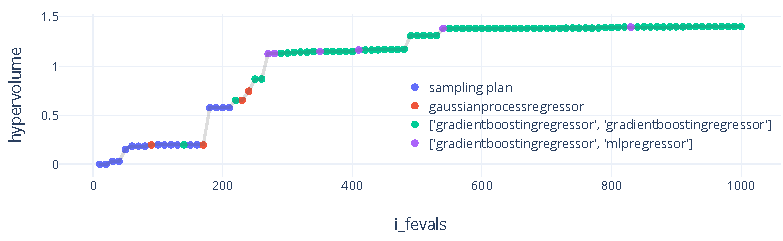
\includegraphics[width=\textwidth]{content/images/dtlz4_models}
            \caption{DTLZ4: Sampling plan bis 210 examples}
            \label{fig:dtlz4_models_210}
        \end{subfigure}
        % \hfill
        
        \begin{subfigure}{\textwidth}
            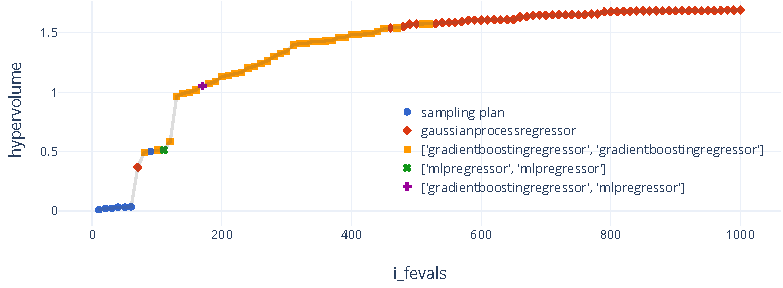
\includegraphics[width=\textwidth]{content/images/wfg1_models}
            \caption{WFG1: Sampling plan bis 60 examples}
            \label{fig:wfg1_models_60}
        \end{subfigure} 

        \caption[The optimization process with dinamic sampling plan and surrogate portfolio.]{The optimization process with dinamic sampling plan and surrogate portfolio. Plots are shown in which step sampling plan was used or which model gives the best accuracy on the test set. More hypervolume is better.}
        \label{fig:changing_models}    
    \end{figure}


    Figure \ref{fig:changing_models} illustrates how improves the solutions for ZDT6 problem. Initially, it could be notest that TutorM considerably outperforms NSGA2 and Hypermapper right from the start of their optimisation process (Fig \ref{fig:zdt6_dist}). TutorM after 300 evaluations, corresponds to the stable near-optimal solution. Besides to interpreter results more involved, non-dominated size should be analysed. ZDT6 landscape has flat regions with local Pareto-front. Hypermapper gets stuck in some of them as evidenced by the serrated graph (Fig \ref{fig:zdt6_ndf}). The drop occurs when discovering a new point in the other Pareto-optimal front. NSGA2 stagnate and comparable to random search due to the many-to-one fitness mapping. Solutions from the population do not have enough sparsity in objective space to detect optimal search direction. TutorM detects global Pareto front straightway and increases Pareto-optimal solutions slowly that alike to solutions from nsga2 with 10k evaluations (Fig \ref{fig:zdt6_front}).

    % === ZDT6
    \begin{figure}
        \centering
        \begin{subfigure}{\textwidth}
            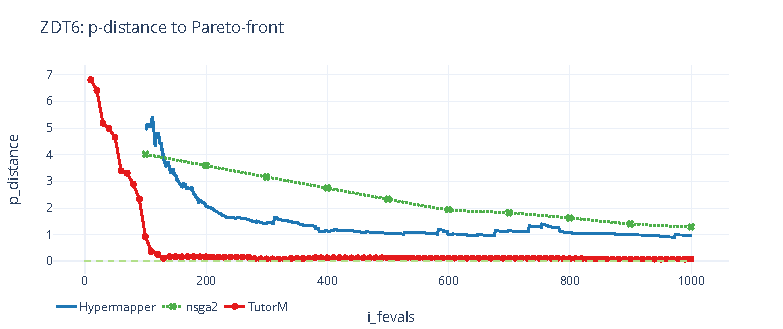
\includegraphics[width=\textwidth]{content/images/zdt6_dist}
            \caption{ZDT6: p-distance to real Pareto-front}
            \label{fig:zdt6_dist}
        \end{subfigure} 
        % \hfill
        
        \begin{subfigure}{\textwidth}
            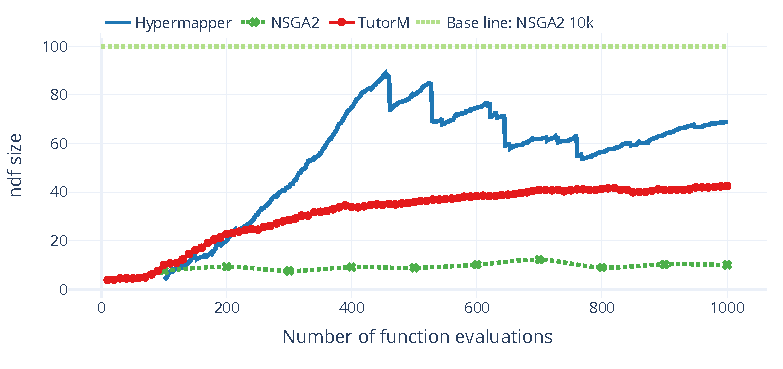
\includegraphics[width=\textwidth]{content/images/zdt6_ndf}
            \caption{ZDT6: Size of a non-dominated subset of an evaluated examples}
            \label{fig:zdt6_ndf}
        \end{subfigure} 

        \begin{subfigure}{\textwidth}
            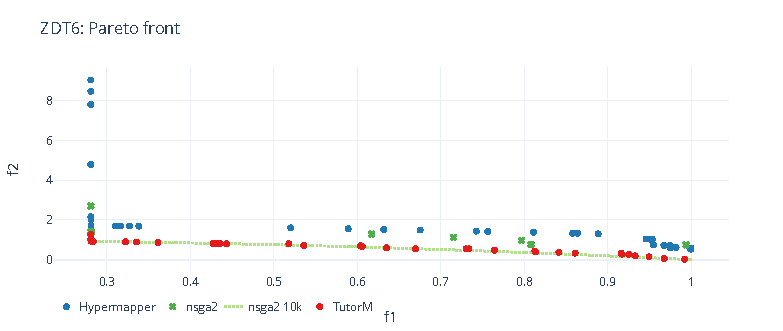
\includegraphics[width=\textwidth]{content/images/zdt6_front}
            \caption{ZDT6: Pareto-front approximation after 1000 function evaluations}
            \label{fig:zdt6_front}
        \end{subfigure} 

        \caption[Comparison of solutions on ZDT6 problem]{A complex comparison of solutions on ZDT6 problem. Final non-dominated points are used to estimate Pareto-optimal solutions.}
        \label{fig:changing_models}    
    \end{figure}


    As shown in Figure \ref{fig:wfg_14}, TutorM could also outperform the MOEA baseline in 10k evaluations(\ref{sub@fig:wfg1_front}). WFG1 has flat landscape regions hence the convergence of genetic algorithms significantly deteriorates. Hypermapper increase count of non-dominated points, regardless it is local optimum and most samples stack in a small region. Nsga2 after 1000 function evaluations also have high-density regions which could be improved with spending more effort to evaluations. The TutorM has several dozen of Pareto-optimal points from all over the budget, that significantly outperforms Hypermapper and nsga2 even with 10k evaluations. 
    From WFG4 use case, all over all approaches gain near-optimal results(\ref{fig:wfg4_front}), but significant advantage over TutorM as it provides an extensive set of points(\ref{fig:wfg4_ndf}) that are well distributed at the Pareto front.


    % === WFG1 and WFG4
    \begin{figure}
        \centering
        \begin{subfigure}{\textwidth}
            \begin{subfigure}{0.5\textwidth}
                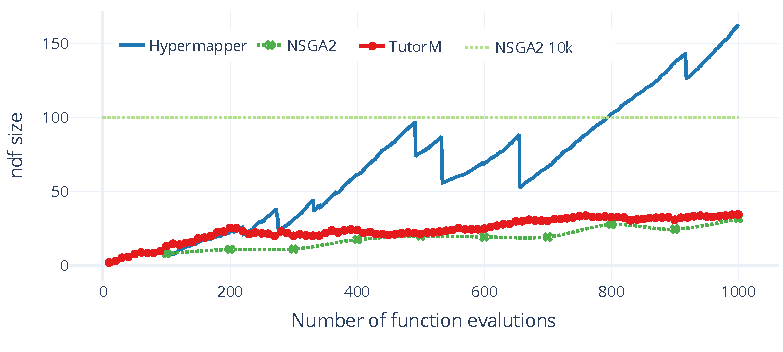
\includegraphics[width=\textwidth]{content/images/wfg1_ndf}
                \caption{WFG1: Size of a non-dominated subset of an evaluated examples}
                \label{fig:wfg1_ndf}
            \end{subfigure} 
            \begin{subfigure}{0.5\textwidth}
                \includegraphics[width=\textwidth]{content/images/wfg1_front}
                \caption{WFG1: Pareto-front approximation}
                \label{fig:wfg1_front}
            \end{subfigure} 
        \end{subfigure} 

        
        % ?\hfill


        \begin{subfigure}{\textwidth}
            \begin{subfigure}{0.5\textwidth}
                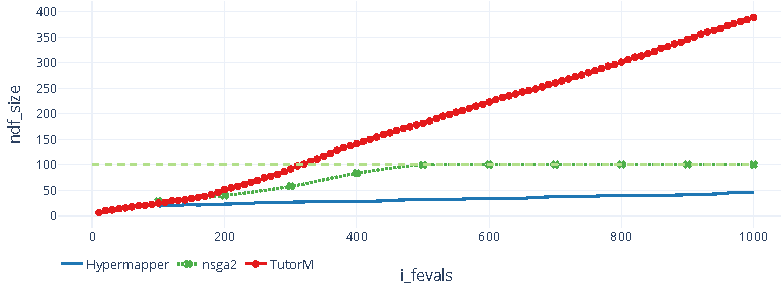
\includegraphics[width=\textwidth]{content/images/wfg4_ndf}
                \caption{WFG4: Size of a non-dominated subset of an evaluated examples}
                \label{fig:wfg4_ndf}
            \end{subfigure} 
            \begin{subfigure}{0.5\textwidth}
                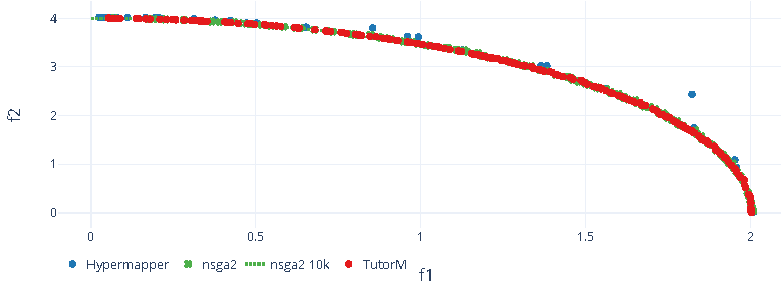
\includegraphics[width=\textwidth]{content/images/wfg4_front}
                \caption{WFG4: Pareto-front approximation}
                \label{fig:wfg4_front}
            \end{subfigure}
        \end{subfigure} 
        
 

        \caption[Comparison of solutions on ZDT6 problem]{A complex comparison of solutions on ZDT6 problem. Final non-dominated points are used to estimate Pareto-optimal solutions.}
        \label{fig:wfg_14}    
    \end{figure}





    \begin{table}[]
        \centering
        \resizebox{\textwidth}{!}{%
        \begin{tabular}{@{}ccccccc@{}}
        \toprule
                                             & \textbf{Metric}        & \textbf{ZDT4} & \textbf{ZDT6} & \textbf{DTLZ4} & \textbf{WFG1} & \textbf{WFG4} \\ \midrule
        \multirow{4}{*}{\textbf{TutorM}}     & \textbf{hypervolume}   & 99,45\%       & 99,01\%       & 99,27\%        & 115,60\%      & 95,95\%       \\
                                             & \textbf{p-distance}    & 1,336         & 0,522         & 0,022          & -             & -             \\
                                             & \textbf{ndf-size}      & 183,022       & 31,528        & 119,308        & 24,158        & 183,244       \\
                                             & \textbf{space-metrics} & 0,103         & 0,142         & 0,186          & 0,129         & 0,032         \\ \midrule
        \multirow{4}{*}{\textbf{NSGA2}}      & \textbf{hypervolume}   & 97,57\%       & 87,46\%       & 95,87\%        & 45,01\%       & 91,87\%       \\
                                             & \textbf{p-distance}    & 1,391         & 1,872         & 0,022          & -             & -             \\
                                             & \textbf{ndf-size}      & 44,000        & 11,455        & 39,900         & 20,164        & 82,436        \\
                                             & \textbf{space-metrics} & 0,176         & 0,355         & 0,268          & 0,228         & 0,038         \\ \midrule
        \multirow{4}{*}{\textbf{Hypermaper}} & \textbf{hypervolume}   & 96,82\%       & 66,95\%       & 81,29\%        & 40,66\%       & 74,09\%       \\
                                             & \textbf{p-distance}    & 2,024         & 1,850         & 0,076          & -             & -             \\
                                             & \textbf{ndf-size}      & 28,908        & 52,746        & 10,743         & 81,512        & 30,158        \\
                                             & \textbf{space-metrics} & 0,1386        & 0,11621       & 0,5282         & 0,0870        & 0,1032        \\ \midrule
        \multirow{4}{*}{\textbf{\begin{tabular}[c]{@{}c@{}}NSGA2\\ 10k eval\end{tabular}}} & \textbf{hypervolume}      & 100,00\% & 100,00\% & 100,00\% & 100,00\% & 100,00\% \\
                                             & \textbf{p-distance}    & 0,152         & 0,256         & 0,002          & -             & -             \\
                                             & \textbf{ndf-size}      & 93,901        & 79,776        & 93,990         & 85,196        & 98,087        \\
                                             & \textbf{space-metrics} & 0,033         & 0,074         & 0,039          & 0,051         & 0,016         \\ \bottomrule
        \end{tabular}%
        }
        \end{table}



    % ======= SUMMARY DTLZ
    % Please add the following required packages to your document preamble:
% \usepackage{booktabs}
% \usepackage{multirow}
% \usepackage{graphicx}
\begin{table}[]
    \centering
    \label{tab:dtlz_summary}
    \resizebox{\textwidth}{!}{%
    \begin{tabular}{@{}llllll@{}}
    \toprule
    \textbf{Problem}                & \textbf{Approach}        & $\downarrow$ \textbf{p-distance} & $\uparrow$ \textbf{Hypervolume} \%  & $\uparrow$ \textbf{ndf size} \% & $\uparrow$  \textbf{ndf space} \\ \midrule
    \multirow{4}{*}{DTLZ1} & Base line       & 0,800           & 100             & 0,24           & 1     \\ \cmidrule(l){2-6} 
    & NSGA2 1k        & \textbf{3,277}  & 56,577          & \textbf{1,56}  & 0,046 \\ \cmidrule(l){2-6} 
    & TutorM          & 51,611          & \textbf{98,163} & 0,54           & 0,058 \\ \cmidrule(l){2-6} 
    & Hypermapper 2.0 & 74,251          & 86,173          & 0,78           & 0,049 \\ \midrule
\multirow{4}{*}{DTLZ2} & Base line       & 5,19e-06        & 98,603          & 0,24           & 0,39 \\ \cmidrule(l){2-6} 
    & TutorM          & \textbf{0,0004} & \textbf{100}    & \textbf{82,56} & 1     \\ \cmidrule(l){2-6} 
    & NSGA2 1k        & 0,003           & 80,415          & 10          & 0,301 \\ \cmidrule(l){2-6} 
    & Hypermapper 2.0 & 0,058           & 76,103          & 2,84           & 0,063 \\ \midrule
\multirow{4}{*}{DTLZ3} & Base line       & 0,4           & 100             & 0,24           & 1     \\ \cmidrule(l){2-6} 
    & NSGA2 1k        & \textbf{4,430}  & 74,937          & 0,82           & 0,037 \\ \cmidrule(l){2-6} 
    & TutorM          & 38,735          & \textbf{97,743} & 0,40           & 0,045 \\ \cmidrule(l){2-6} 
    & Hypermapper 2.0 & 92,228          & 95,010          & 0,70           & 0,047 \\ \midrule
\multirow{4}{*}{DTLZ4} & Base line       & 8,81e-06        & 100             & 0,36           & 1     \\ \cmidrule(l){2-6} 
    & TutorM          & \textbf{0,001}  & \textbf{99,829} & \textbf{30,68} & 0,666 \\ \cmidrule(l){2-6} 
    & NSGA2 1k        & 0,002           & 87,807          & 9,60           & 0,323 \\ \cmidrule(l){2-6} 
    & Hypermapper 2.0 & 0,059           & 64,579          & 1,18           & 0,029 \\ \midrule
\multirow{4}{*}{DTLZ5} & Base line       & 1,62e-05        & 98,631          & 0,24           & 0,486 \\ \cmidrule(l){2-6} 
    & TutorM          & \textbf{0,0004} & \textbf{100}    & \textbf{80,88} & 1     \\ \cmidrule(l){2-6} 
    & NSGA2 1k        & 0,002           & 81,729          & 10          & 0,434 \\ \cmidrule(l){2-6} 
    & Hypermapper 2.0 & 0,058           & 78,463          & 3,02           & 0,06 \\ \midrule
\multirow{4}{*}{DTLZ6} & Base line       & 0,009           & 100             & 0,24           & 1     \\ \cmidrule(l){2-6} 
    & TutorM          & \textbf{0,123}  & \textbf{98,064} & 3,70           & 0,142 \\ \cmidrule(l){2-6} 
    & NSGA2 1k        & 1,011           & 54,258          & 2,88           & 0,128 \\ \cmidrule(l){2-6} 
    & Hypermapper 2.0 & 1,657           & 18,355          & 2,22           & 0,084 \\ \midrule
\multirow{4}{*}{DTLZ7} & Base line       & 2,42e-07        & 99,938          & 0,24           & 0,364 \\ \cmidrule(l){2-6} 
    & TutorM          & \textbf{0,0003} & \textbf{100}    & \textbf{87} & 1     \\ \cmidrule(l){2-6} 
    & NSGA2 1k        & 0,160           & 92,891          & 3,04           & 0,128 \\
    & Hypermapper 2.0 & 0,781           & 91,129          & 2,24           & 0,081 \\ \cmidrule(l){2-6} 
\end{tabular}%
    }
    \caption{DTLZ problem set: Comparison between Hypermapper 2, NSGA2 and TutorM.  All Results were averaged after 5 reps with a 1,000 evaluations budget.
    The general baseline is the NSGA2 with 50k evaluations (100 population size in 500 generations)}
    \end{table}



    % ======= SUMMARY ZDT
    % Please add the following required packages to your document preamble:
% \usepackage{booktabs}
% \usepackage{multirow}
% \usepackage{graphicx}
\begin{table}[]
    \centering
    \resizebox{\textwidth}{!}{%
    \begin{tabular}{@{}llllll@{}}
    \toprule
    \textbf{Problem}                & \textbf{Approach}        & $\downarrow$ \textbf{p-distance} & $\uparrow$ \textbf{Hypervolume} \%  & $\uparrow$ \textbf{ndf size} \% & $\uparrow$  \textbf{ndf space} \\ \midrule
    \multirow{4}{*}{ZDT1} & Base line       & 1,08e-05          & 99,78          & 0,16           & 0,22          \\ \cmidrule(l){2-6} 
                          & TutorM          & \textbf{4,74e-05} & \textbf{100}   & \textbf{90,33} & \textbf{1}    \\ \cmidrule(l){2-6} 
                          & NSGA2 1k        & 0,02              & 89,86          & 9,66           & 0,08          \\ \cmidrule(l){2-6} 
                          & Hypermapper 2.0 & 0,12              & 98,93          & 10,36          & 0,04          \\ \midrule
    \multirow{4}{*}{ZDT2} & Base line       & 1,04e-14          & 99,79          & 0,16           & 0,29          \\ \cmidrule(l){2-6} 
                          & TutorM          & \textbf{0,00013}  & \textbf{100}   & \textbf{86,87} & \textbf{1}    \\ \cmidrule(l){2-6} 
                          & NSGA2 1k        & 0,01              & 88,78          & 8,82           & 0,06          \\ \cmidrule(l){2-6} 
                          & Hypermapper 2.0 & 0,18              & 97,31          & 5,12           & 0,04          \\ \midrule
    \multirow{4}{*}{ZDT3} & Base line       & 1,69e-08          & 100            & 0,16           & 0,39          \\ \cmidrule(l){2-6} 
                          & TutorM          & \textbf{0,00012}  & \textbf{99,47} & \textbf{86}    & \textbf{1}    \\ \cmidrule(l){2-6} 
                          & NSGA2 1k        & 0,02              & 89,92          & 9,82           & 0,28          \\ \cmidrule(l){2-6} 
                          & Hypermapper 2.0 & 0,31              & 92,03          & 5,64           & 0,12          \\ \midrule
    \multirow{4}{*}{ZDT4} & Base line       & 2,04e-05          & 100            & 0,72           & 1             \\ \cmidrule(l){2-6} 
                          & TutorM          & \textbf{0,01}     & \textbf{99,80} & \textbf{50,0}  & \textbf{0,78} \\ \cmidrule(l){2-6} 
                          & NSGA2 1k        & 0,04              & 83,43          & 8,77           & 0,19          \\ \cmidrule(l){2-6} 
                          & Hypermapper 2.0 & 0,90              & 97,32          & 5,42           & 0,11          \\ \midrule
    \multirow{4}{*}{ZDT6} & Base line       & 0,0003            & 100            & 0,72           & 1             \\ \cmidrule(l){2-6} 
                          & TutorM          & \textbf{0,09}     & \textbf{99,43} & 4,26           & 0,17          \\ \cmidrule(l){2-6} 
                          & Hypermapper 2.0 & 1,12              & 82,86          & \textbf{6,25}  & 0,08          \\ \cmidrule(l){2-6} 
                          & NSGA2 1k        & 1,29              & 83,84          & 1,01           & 0,04          \\ \bottomrule
    \end{tabular}%
    }
    \caption{ZDT problem set: Comparison between Hypermapper 2, NSGA2 and TutorM.  All Results were averaged after 5 reps with a 1,000 evaluations budget.
    The general baseline is the NSGA2 with 50k evaluations (100 population size in 500 generations)}
    \label{tab:zdt_sumaary}
    \end{table}


    % ======= SUMMARY WFG
    % Please add the following required packages to your document preamble:
% \usepackage{booktabs}
% \usepackage{multirow}
% \usepackage{graphicx}
\begin{table}[]
    \centering
    \resizebox{!}{11cm}{%
    \begin{tabular}{@{}lllll@{}}
    \toprule
    \textbf{Problem}                & \textbf{Approach}        & $\uparrow$ \textbf{Hypervolume} \%  & $\uparrow$ \textbf{ndf size} \% & $\uparrow$  \textbf{ndf space} \\ \midrule
    \multirow{4}{*}{WFG1} & Base line       & 100            & 0,72           & 1             \\ \cmidrule(l){2-5} 
                          & TutorM          & \textbf{95,75} & 3,44           & \textbf{0,51} \\ \cmidrule(l){2-5} 
                          & Hypermapper 2.0 & 44,12          & \textbf{10,24} & 0,31          \\ \cmidrule(l){2-5} 
                          & NSGA2 1k        & 30,52          & 3,18           & 0,28          \\ \midrule
    \multirow{4}{*}{WFG2} & Base line       & 100            & 0,08           & 0,63          \\ \cmidrule(l){2-5} 
                          & TutorM          & \textbf{98,64} & \textbf{29,22} & \textbf{1}    \\ \cmidrule(l){2-5} 
                          & NSGA2 1k        & 85,96          & 6,44           & 0,35          \\ \cmidrule(l){2-5} 
                          & Hypermapper 2.0 & 62,35          & 1,20           & 0,10          \\ \midrule
    \multirow{4}{*}{WFG3} & TutorM          & \textbf{100}   & \textbf{55,50} & \textbf{1}    \\ \cmidrule(l){2-5} 
                          & Base line       & 99,05          & 0,08           & 0,29          \\ \cmidrule(l){2-5} 
                          & NSGA2 1k        & 84,46          & 9,72           & 0,15          \\ \cmidrule(l){2-5} 
                          & Hypermapper 2.0 & 73,31          & 2,44           & 0,02          \\ \midrule
    \multirow{4}{*}{WFG4} & Base line       & 100            & 0,72           & 0,60          \\ \cmidrule(l){2-5} 
                          & TutorM          & \textbf{99,28} & \textbf{38,90} & \textbf{1}    \\ \cmidrule(l){2-5} 
                          & Hypermapper 2.0 & 84,39          & 3,26           & 0,06          \\ \cmidrule(l){2-5} 
                          & NSGA2 1k        & 83,95          & 10             & 0,58          \\ \midrule
    \multirow{4}{*}{WFG5} & Base line       & 100            & 0,20           & 0,24          \\ \cmidrule(l){2-5} 
                          & TutorM          & \textbf{98,01} & \textbf{87,60} & \textbf{1}    \\ \cmidrule(l){2-5} 
                          & Hypermapper 2.0 & 84,83          & 34,74          & 0,06          \\ \cmidrule(l){2-5} 
                          & NSGA2 1k        & 82,70          & 10,00          & 0,18          \\ \midrule
    \multirow{4}{*}{WFG6} & TutorM          & \textbf{100}   & \textbf{52,68} & \textbf{1}    \\ \cmidrule(l){2-5} 
                          & Base line       & 99,30          & 0,20           & 0,33          \\ \cmidrule(l){2-5} 
                          & NSGA2 1k        & 86,59          & 10             & 0,27          \\ \cmidrule(l){2-5} 
                          & Hypermapper 2.0 & 83,21          & 2,36           & 0,03          \\ \midrule
    \multirow{4}{*}{WFG7} & TutorM          & \textbf{100}   & \textbf{46,30} & \textbf{1}    \\ \cmidrule(l){2-5} 
                          & Base line       & 99,30          & 0,20           & 0,33          \\ \cmidrule(l){2-5} 
                          & NSGA2 1k        & 86,39          & 10             & 0,26          \\ \cmidrule(l){2-5} 
                          & Hypermapper 2.0 & 83,14          & 2,36           & 0,04          \\ \midrule
    \multirow{4}{*}{WFG8} & Base line       & 100            & 0,20           & 1             \\ \cmidrule(l){2-5} 
                          & TutorM          & \textbf{95,24} & \textbf{20,70} & \textbf{0,26} \\ \cmidrule(l){2-5} 
                          & Hypermapper 2.0 & 86,74          & 2,80           & 0,07          \\ \cmidrule(l){2-5} 
                          & NSGA2 1k        & 79,63          & 9,54           & 0,20          \\ \midrule
    \multirow{4}{*}{WFG9} & Base line       & 100            & 0,20           & 0,85          \\ \cmidrule(l){2-5} 
                          & TutorM          & \textbf{92,17} & \textbf{12,92} & \textbf{0,63} \\ \cmidrule(l){2-5} 
                          & Hypermapper 2.0 & 80,80          & 7,30           & 0,24          \\ \cmidrule(l){2-5} 
                          & NSGA2 1k        & 73,56          & 10             & 1             \\ \bottomrule
    \end{tabular}%
    }
    \caption{WFG problem set: Comparison between Hypermapper 2, NSGA2 and TutorM.  All Results were averaged after 5 reps with a 1,000 evaluations budget.
    The general baseline is the NSGA2 with 50k evaluations (100 population size in 500 generations)}
    \label{tab:wfg_summary}
    \end{table}


    



% --------------------------------------------------------------------------------------------
% ---------------------       Benchmark 2: Dynamic sampling plan and parameter selection
% --------------------------------------------------------------------------------------------
\section{Benchmark 2: Inner parameters}
    Inner parameter tuning is also a problem that should be explained. Whereas in related work, there is not enough information about how to configure model-based parameter tuning. In benchmark-2, we compare different combinations of hyperparameters to define the correlation and importance of those. Due to limited time, we consider only ZDT4 problem  and with a surrogate portfolio from the previous benchmark, but without the Gaussian regression model. Evaluation budget and experiment repeated stayed the same.


    The following options are highlighted in the developed TutorM class:
    \begin{itemize}
        \item Initial dataset [0, 100, 500, 750]
        \item Validation
            \begin{itemize}
                \item Train/test split [75/25, 90/10]
                \item Cross-Validation threshold [0.2, 0.65, 0.9]
                \item Test threshold [0, 0.6, 0.9]
            \end{itemize}
        \item Optimization search algorithm [NSGA2, MOEA-Ctrl]
        \item Pareto front infill-criteria. Solution combinations [Non-dominated front score, Stacking]
        \item Prediction count [10, 100]
    \end{itemize}

    As a result, was done full factorial design with 576 possible configurations and spend almost 2 weeks for 5 repetitions.

    On the Figure shown result for 40 best and worst configurations. Note that the main impact on the quality of the final results gain from solution combination from valid surrogates models. In the case of a $ndf_score$, for final prediction selected optimal points from the surrogate model that has the highest score on non-dominated points from the test set. From another hand, stacking, as an alternative approach, means combining solutions from all models that pass validation, not only from the best one.

    The $ndf_score$  was common to all configurations that gave the worst result, while stacking is preferred choice for best configuration group. Another fascinating conclusion could be done from the initial sample size. Worst parameters involved only empty and 100 initial sets that are reasonable because the lower limit for the worst possible result is higher with more extensive data set. But at the same time, the lack of initial samples yields the best results. If so, the optimization process could begin earlier and achieve the optimum faster. 

    It is also specified to note a tendency to decrease the test threshold, so which is confirmed not to apply general accuracy as the main criteria for surrogate selection.

    % ===  ------------------------------------- ZDT6
    \begin{figure}
        \centering
        \begin{subfigure}{\textwidth}
            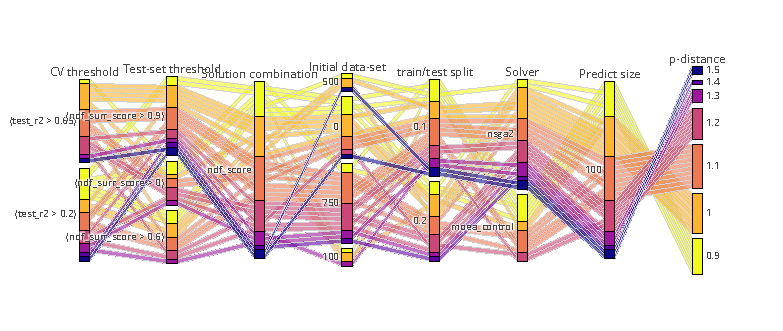
\includegraphics[width=\textwidth]{content/images/conf_zdt6_worst}
            \caption{40 worst configurations}
            \label{fig:conf_zdt6_worst}
        \end{subfigure} 
        % \hfill
        
        \begin{subfigure}{\textwidth}
            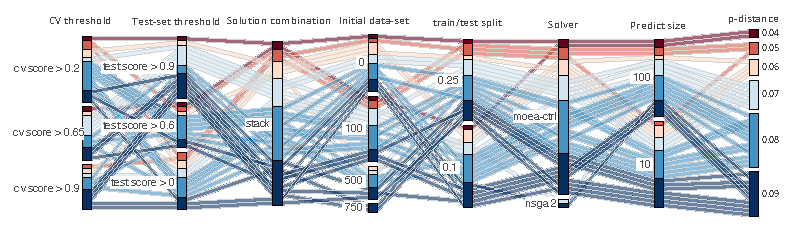
\includegraphics[width=\textwidth]{content/images/conf_zdt6_best}
            \caption{40 best configurations}
            \label{fig:conf_zdt6_best}
        \end{subfigure} 

        \caption[ZDT6: The selection from average result of best and worst configurations.]{ZDT6: The selection from average result of best and worst configurations.}
        \label{fig:conf_zdt6}    
    \end{figure}

    % === ZDT 6
    \begin{figure}
        \centering

        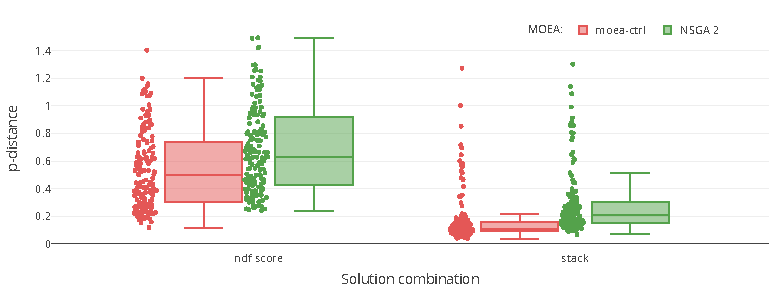
\includegraphics[width=\textwidth]{content/images/conf_zdt6_solver}

        \caption[Correlation between the most influenceable parameters for the ZDT4]{Correlation between the most influenceable parameters for the ZDT6: solution combination strategy and optimization algorithm}
        \label{fig:conf_zdt6}    
    \end{figure}


    % === -------------------------------------- ZDT 4
    \begin{figure}
        \centering
        \begin{subfigure}{\textwidth}
            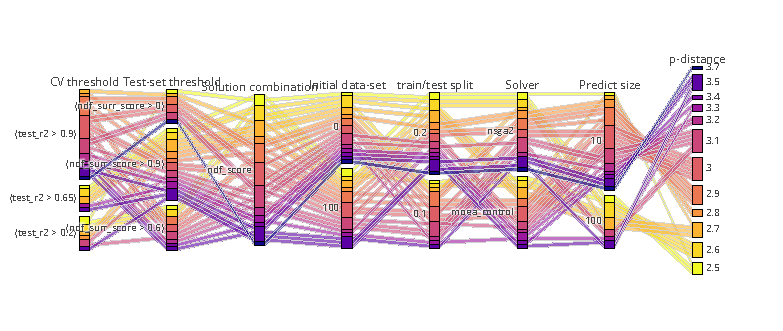
\includegraphics[width=\textwidth]{content/images/conf_zdt4_worst}
            \caption{ZDT4: worst configurations}
            \label{fig:conf_zdt4_worst}
        \end{subfigure} 
        \hfill
        
        \begin{subfigure}{\textwidth}
            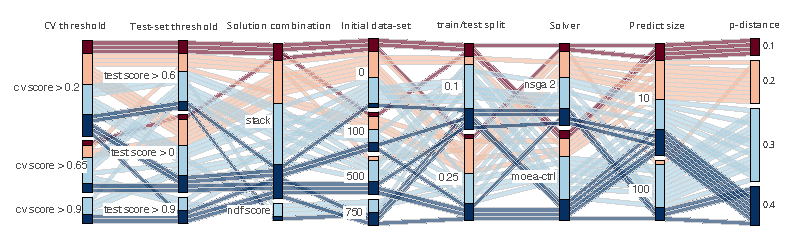
\includegraphics[width=\textwidth]{content/images/conf_zdt4_best}
            \caption{ZDT4: best configurations}
            \label{fig:zdt6_ndf}
        \end{subfigure} 

        \caption[ZDT4: The selection from average result of best and worst configurations.]{ZDT4: The selection from average result of best and worst configurations.}
        \label{fig:conf_zdt4_best}    
    \end{figure}

    % === ZDT4
    \begin{figure}
        \centering

        \begin{subfigure}{\textwidth}
            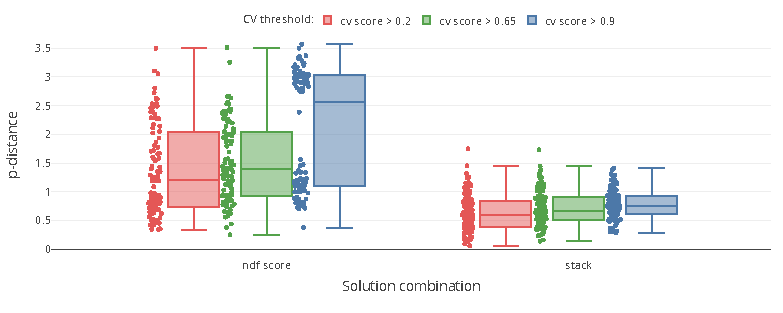
\includegraphics[width=\textwidth]{content/images/conf_zdt4_cv_score}
            \caption{An impact of the cross-validation's threshold}
            \label{fig:zdt4_pred_solver}
        \end{subfigure} 
        \begin{subfigure}{\textwidth}
            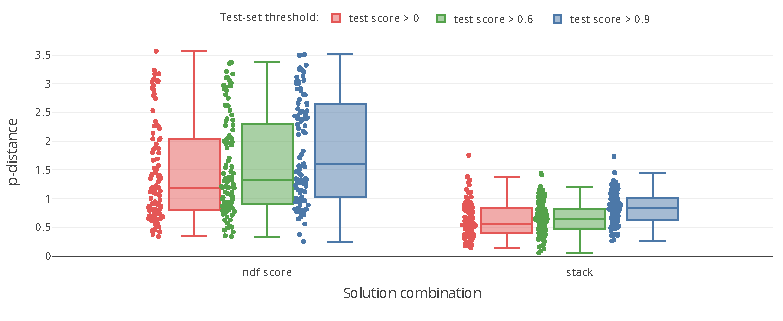
\includegraphics[width=\textwidth]{content/images/conf_zdt4_test_score}
            \caption{An impact of the test-set-validation's threshold}
            \label{fig:zdt4_comb_valid}
        \end{subfigure}

        \caption[Correlation between the most influenceable parameters for the ZDT4]{Correlation between the most influenceable parameters for the ZDT4} 
        \label{fig:conf_zdt6}    
    \end{figure}


    %! [ Hypermapper baseline; ModelTutor and change quality (grid plot)] iterations

    %! [ Hypermapper baseline; ModelTutor and change quality (bubble chart) ] Deviations



% --------------------------------------------------------------------------------------------
% ---------------------       Benchmark 3: Many-objective optimization, scaling
% --------------------------------------------------------------------------------------------
\section{Benchmark 3: Many-objective optimization. Scaling. RQ1.1}

    The goal of this experiment is to find out the scalability of surrogate models. Compositional models build faster but could be not accurate enough. The GausionProcess regression properties are opposite - good surface approximation requires much time. 

    For evaluation scalability property for the compositional model, was selected highly multimodal DTLZ1 problem. Problem dimensionality is fixed and scale objectives.



    % For evaluation scalability property for the compositional model, problem XXX was selected.

    % Objectives: 1) detect iterative improvement, a convergence of the primary metric 2) time for evaluation

    % Usecases: GausianModel, GausianModel + Gradient, GausianModel + random forest, 

    % Scale: objectives - 2,4,8,10; params - 2,4,8,10

    % ! [ Hypermapper baseline; X - objectives Y - p-distance/time]



% --------------------------------------------------------------------------------------------
% ---------------------       Benchmark 4: real world scenario
% --------------------------------------------------------------------------------------------
% \section{Benchmark 4: Parameter tuning of SVM}

%     % ! [ Hypermapper baseline; SVM score in iterations]


% --------------------------------------------------------------------------------------------
% ------------------------------------------------     Discussion 
% --------------------------------------------------------------------------------------------
\section{Discussion}

Up to now, most papers used the
The quality of the results obtained with X was similar to the results obtained with Y, but with significantly fewer exactly evaluated solutions during the optimization process. 


consume an inordinate amount of time.

% Discussion

% non-separable
% or have a deceptive fitness landscape

% However, GAs, or at least some variants of them, are not 100'\%' ruled out.

% +’, ’−’ and ’≈’, which indicate that the result is significantly better, significantly worst and statistically similar to the result in the control column, respectively. 


% On the left side the learning curve of a naive Bayes classifier is shown for the digits dataset. Note that the training score and the cross-validation score are both not very good at the end. However, the shape of the curve can be found in more complex datasets very often: the training score is very high at the beginning and decreases and the cross-validation score is very low at the beginning and increases. On the right side we see the learning curve of an SVM with RBF kernel. We can see clearly that the training score is still around the maximum and the validation score could be increased with more training samples.
% https://scikit-learn.org/0.15/auto_examples/plot_learning_curve.html




% Compared to Auto-WEKA, this is much more data-efficient: in
% Auto-WEKA, evaluating the performance of an ensemble with 5 components requires the construction
% and evaluation of 5 models; in contrast, in auto-sklearn, ensembles come largely for free, and it is
% possible to mix and match models evaluated at arbitrary times during the optimization.


% This makes the archive gradually move towards the Pareto-front.
% 80% of the computing-time is spent in the area close to the Pareto front.


% We would like to prove that the use of hierarchical surrogates has a higher probability to find the optimum of the optimization problem in Eq. (4) ref[Evolutionary optimization with hierarchical surrogates]


% Test problems ZDT1, ZDT2, and ZDT3 show a different trend in function evaluations as compared to OSY.


% In contrast to PR, ANN, RBF, GP, Ranking SVM is invariant to